% TEX root = ../Thesis.tex
\chapter{Introduction}

\newchapter{R}{esearch has shown} that climate change is a fact, and with a 95\% certainty that human activity is the main cause for global warming \fcite{ipcc2013climate}. As a way to mitigate the increasing rate of climate change, the previous Danish government \bondy{cabinet} has set as an interim goal to reduce the national $CO_2$ emissions by 40\% in 2020, in order to reach the target of 80\% - 95\% reduction by 2050\fcite{regeringen2013danish}. This is to be done by covering 50\% of the national electricity consumption with wind energy by 2020, fully covering the electricity and heating supply with renewable energy by 2035, and being completely fossil fuel independent by 2050. Investing in a intelligent and flexible power system is deemed to be important if we are to reach those goals\fcite{regeringen2013smart}.

Although the government \bondy{cabinet}\todo{Check with Henrik what should be the correct wording here} changed in 2015 and the financial support to environmentally friendly initiatives was significantly reduced, we still consider the previously established goals worth pursuing, as explained in Section~\ref{sec:justification}. In order to integrate the wind generated energy into the power system, the power system must change as described in Section~\ref{sec:powsysdesc}. In Section~\ref{sec:funneling} challenges are identified within this new power system framework, and this work's contributions to solve said challenges are summarized.
%adopted by the Danish government, a large part of Danish research has been focused on how to integrate renewable energy sources, as well as new distributed energy resources, into the power system. The world energy sector is experiencing drastic changes due to environmental, health and security issues. 
\section{On the justification of research in renewable generation} % (fold)
\label{sec:justification}

\newsection{E}{nergy is a pillar} in the development of all countries. The access to energy is a necessity that traditionally is supplied by fossil fuels. The use of fossil fuels has been one of the main contributors to the $CO_2$ emissions that impact the climate. This has lead to research in the area of renewable energy sources.

Governments around world are taking steps to mitigate their vulnerability in energy supply.
\begin{itemize}
	\item The climate question - The Brundtland report
	\item Health issues/pollution
	\item Energy security, cite the paper The concept of energy security: Beyond the four As by Cherp and Jewell
\end{itemize}

% section justification (end)


\section{Changes in the power system}% (fold)
\label{sec:powsysdesc}
\newsection{I}{n order to understand} \marginnote{This section is partially based on a technical report prepared for the iPower project \cite{bondy2014a}, as well as the popular science paper presented for the course 31920, Communicating Advanced topics in Electrical Engineering.} the relevance of this research project, it is important to define how we expect the power system to change, and clarify what is the frame for the research. This section gives a general introduction\footnote{In-depth explanations will be presented as needed in subsequent chapters.} to the changes expected in the power system. The main actors in the power system and their relationships are presented, which will help scoping the problem.
\subsection*{The Traditional Power System: Produce as we Consume}
\label{sub:traditional}
\marginnote{This subsection is intended for readers who are not already familiar with the power system. It clarifies basic concepts such as production/consumption balance, system frequency, system operators, energy markets, etc.}
The goal of the power system is to provide an adequate and secure electricity supply to the population.
The electric power system today is composed of two layers (Figures~\ref{fig:powernow}-\ref{fig:marketnow}): 
\begin{description}
	\item[Physical grid] This is the level at which the electricity flows, going from generators to transmission system, to distribution system and finally to the end consumer.
	\item[Market layer] This is where all the energy trade and business operations are made. This includes the sale of electricity from producers to \glspl{brc}. Retailers in turn buy electricity from the BRCs and sell it to the end consumer. Being a \gls{brp}, either as a consumer or as a producer, means that the actor is responsible for its own forecasts and must ensure the best possible that the actual production/consumption follows the planned schedules.
\end{description}

\begin{figure}[t]
	\centering
	\caption{The Electric Power System as seen today. The power generated is first transmitted at high voltage levels to industrial consumers and transformer substations, from where it is distributed at medium/low voltage to medium size consumers and households.}\label{fig:powernow}
	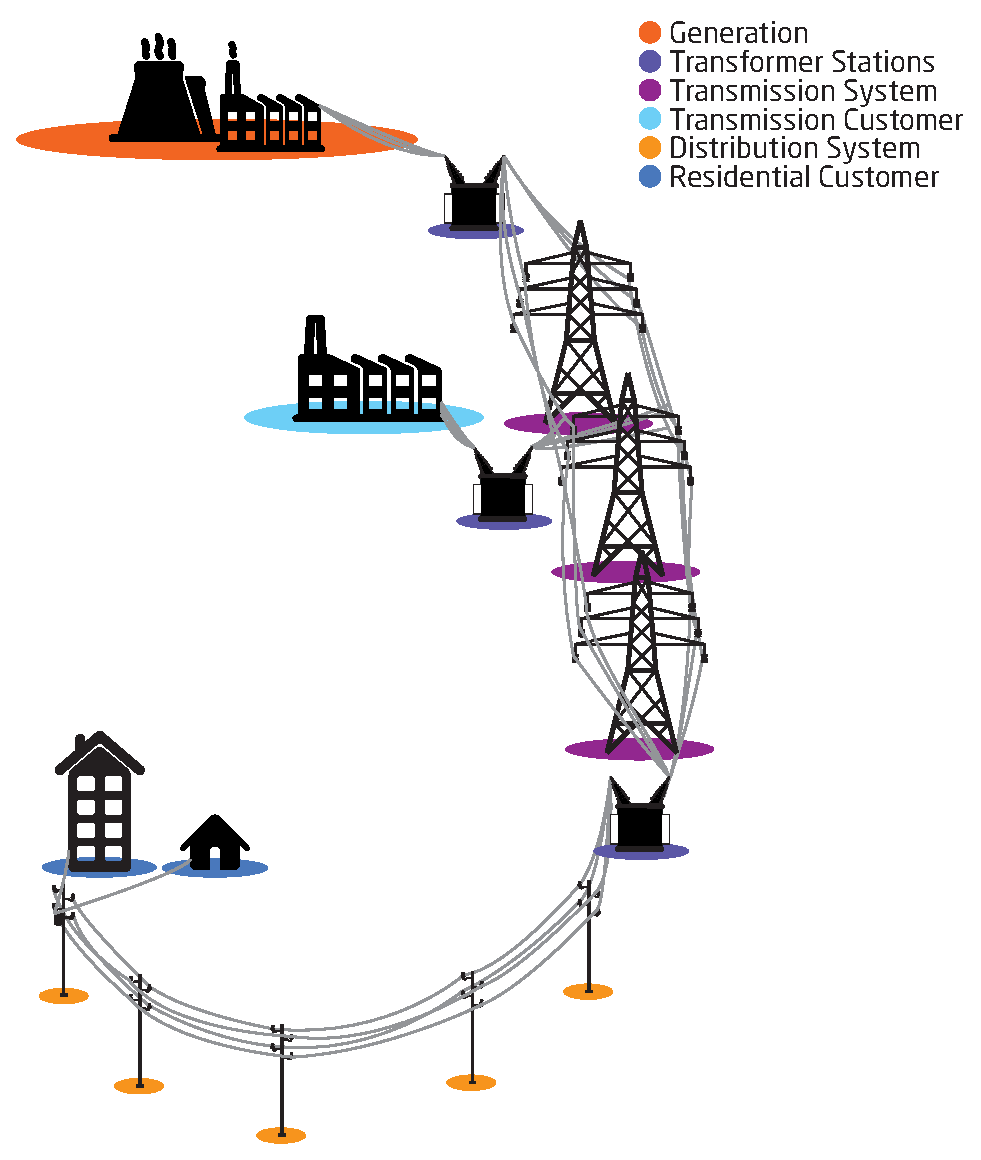
\includegraphics[width=\textwidth]{intro/traditional_grid_new.eps}
\end{figure}

While market regulations can be adjusted or completely changed in order to cope with the large influx of renewable energy, the physical laws cannot.
When electricity is produced it must also be consumed. With current technology it is unfeasible to store electricity in large quantities, therefore electricity companies must forecast how much electricity consumers are going to need the next day and then buy electricity accordingly. I.e., the production of electricity must match the consumption of electricity. If there is a surplus of electricity in the system (production exceeds consumption), the system frequency increases\sidenote[][-3\baselineskip]{The system frequency is a measure of the balance of the grid. Electricity is traditionally produced with turbines which rotate synchronously in a given area. The system frequency, e.g. 50 Hz in Europe, is a measure of the balance of the system, with higher frequencies signaling a power surplus and lower frequencies signaling power deficit in the system.}%\todo{Check up on sources}}
, and might eventually damage electric components in the grid. Vice versa, a deficiency of electricity in the system (consumption exceeds production) can lead to a blackout. 
\begin{figure*}[htbp!]
		\centering
		\caption{The actors and relationships in the power market today. Note that the consumer buys electricity from a retailer, but has no further contact to the other market actors, i.e. the consumer has a passive role in the system.}\label{fig:marketnow}
	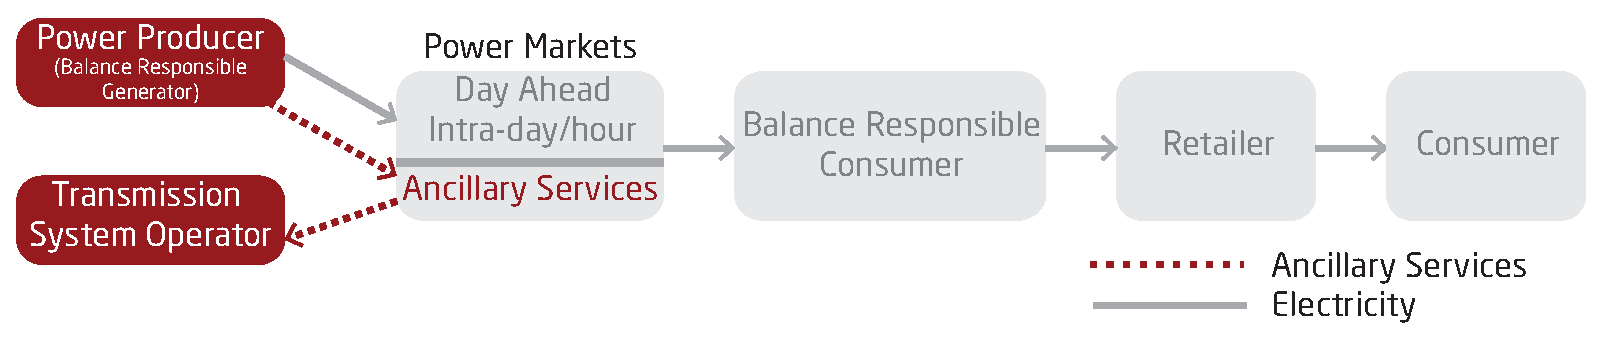
\includegraphics[width=0.8\textwidth]{intro/market_now.eps}
\end{figure*}

The consumption forecasts are imperfect, which leads to a constant imbalance between production and consumption of electricity. The \gls{tso} is the entity responsible of resolving the imbalances of the system and maintaining the secure operation of the system. In order to do this, the TSO buys ancillary services from \emph{certified generators}\footnote[][-2\baselineskip]{The concept of certification of units to deliver ancillary services is central to this work and will be expanded upon in Chapter~\ref{cha:validation}.}  through the ancillary service markets. This market relationship is also reflected in Figure~\ref{fig:marketnow}. There are different types of services, and thorough overviews and explanations of these can be found in the literature\fcite{entso1operational,Rebours}. Here it suffices to say\footnote{Further discussion on ancillary services will be presented in Chapter~\ref{cha:services}.} that for most ancillary services, the TSO will pay generators to deviate from their planned production plans in order to bring the system back to balance. In the future, it is expected that the traditional sources of ancillary services, i.e. large central fossil-fuel powered generation plants, will be outphased in favor of smaller distributed and renewable generation. This means that new sources for ancillary services must be found.  

\subsection*{The New Flexible Power System: Consume as we Produce}
\label{sub:future}
In the traditional power system, the uncertainty in consumption causes imbalances. With the increase of wind energy and solar generation, the uncertainty traditionally only associated with consumption spreads to the production side. Furthermore, traditional sources of ancillary services are closing down, which means that TSOs must find new ways of balancing the system. Also, new problems will appear at the distribution system level, such as power congestion and voltage issues. These problems arise because of new consumption technologies appearing in the system, such as \glspl{ev} and \glspl{hp}, and because of new generation units, \eg \glspl{wt}, small size \glspl{chp} and \glspl{pv}, are installed at distribution level. All these new units in the electric power system are commonly referred to as \glspl{der}\footnote{In this work the concept of DER includes \gls{dg}, \gls{ee}, demand response (DR) and \gls{dess}, which is a combination of the the traditional definition of DER = DG + DESS (as seen in \eg \cite{nrel2002using}) and the broader definition presented in \cite{nys2014reforming}.} or flexible resources. It is the responsibility of the \gls{dso} to resolve the problems arising due to the integration of the DERs, which can be the overloading of system components or voltage issues. These problems affect the quality of the power supply at residential level, but can also lead to issues at transmission level.
\begin{figure}[ht]
	\centering
	\caption{The Electric Power System of tomorrow contains a large ICT infrastructure, which permits the flow of information and control between the system actors. Furthermore, the flow of electricity is not only from generator to consumer, but there is also intermittent electricity generation at distribution level.}
	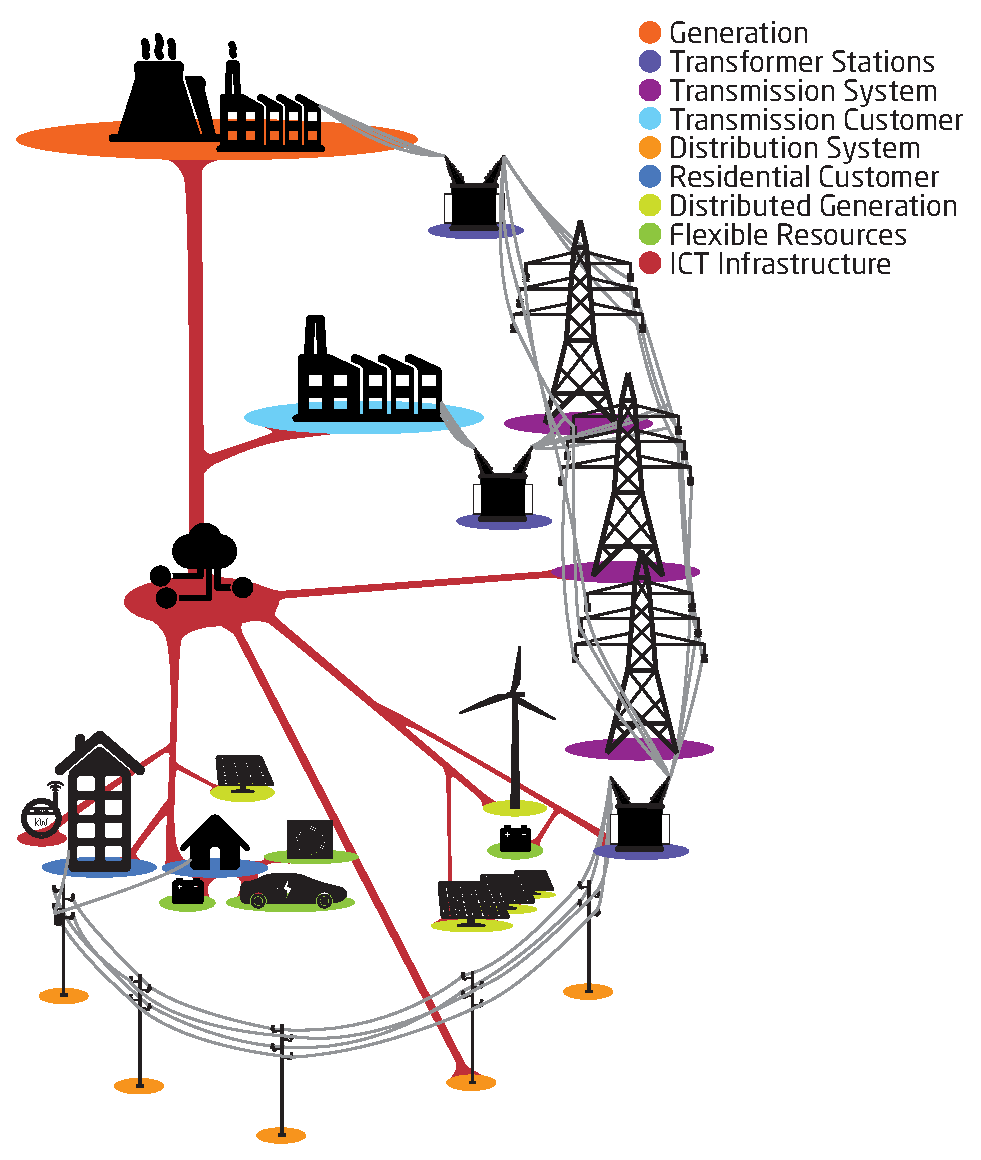
\includegraphics[width=\textwidth]{intro/smart_grid_new.eps}\label{fig:powerfuture}
\end{figure}

The expected future smart grid can be seen in Figure~\ref{fig:powerfuture}, where not only the new DERs appear but an \Gls{ict} infrastructure coordinates the behaviour of the units for the benefit of the system. Smart metering is added at consumer level, and sensors are deployed at distribution level.
\begin{figure*}[htbp!]
	\centering
	\caption{The actors and relationships in the power market of tomorrow. Compared to the current market setup, the aggregator entity has been added, as well as the ability of DSOs to contract services from the aggregator. The aggregator delivers ancillary services to the TSO through a BRC. Also, the consumer becomes a player in the electricity markets through the aggregator.}
	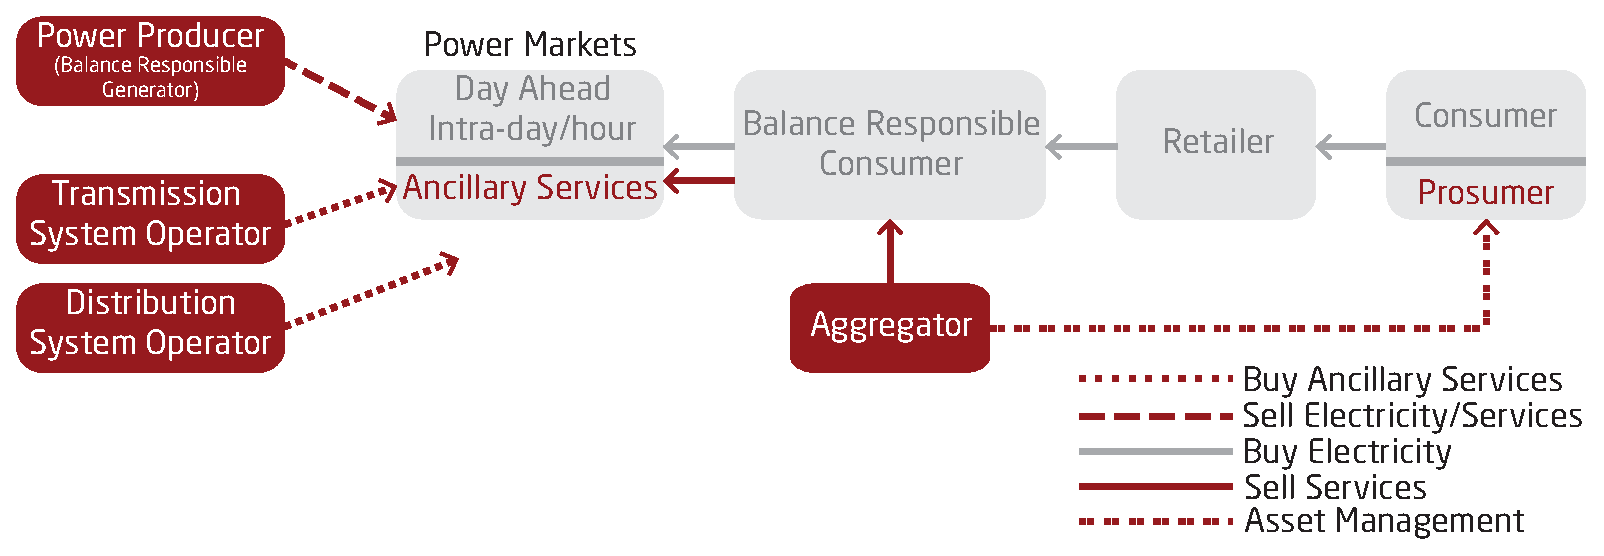
\includegraphics[width=0.8\textwidth]{intro/market_future.eps}\label{fig:marketfuture}
\end{figure*}

In order to cope with the new problems, both at transmission and distribution level, it is expected that consumers will become prosumers. That is, the consumers will take an active role in the power markets by selling services to the system operators through an aggregator\footnote{The concept of the aggregator is further discussed in Chapter~\ref{cha:aggregator}.}. The aggregator will provide an asset management service to the end consumer, and by managing a pool of consumers, it will be able to control a large enough consumption volume to provide ancillary services to the system operators, or balancing services to the consumption BRP. The action of a consumer changing his or her consumption based upon an incentive is known as \gls{dr}. The aggregator facilitates DR by providing the ICT infrastructure and control infrastructure to DER owners, as well as statistical certainty of service delivery and legal responsibility towards the system operators. The aggregator can be an independent commercial entity, or it can be a function inside one of the pre-existing market players. The new market setup can be seen in Figure~\ref{fig:marketfuture}, and it shows how the aggregator entity will interact with the existing market setup, and how the DSO will become a new player in the market, which will acquire services to resolve some of it problems.

In conclusion, we see the electric power system moving away from a \emph{production-must-follow-consumption} pattern to \emph{consumption-should-partly-follow-production} and hereby facilitate the integration of renewables and DERs. An integral part of achieving this change will be the use of control services to change the consumption behavior of units in the network. Given that the units providing ancillary services to the grid are critical for the security of the system, system operators must be able to trust that the units will behave as required. This is ensured by validating the new control algorithms and infrastructure through tests.



\todo{amplify the paper to contain an analogy of the frequency as inflow and outflow of a water tank}
% section Short introduction to the power system (end)

\section{Problem statement, Delimitation and Contributions} % (fold)
\label{sec:Funneling}
\newsection{W}{hat is meant by} control-services? This is a broad definition, and here I will  narrow down my research to use control services to provide ancillary services, primarily through demand response, but the techniques should be able to be generalized.

Scoping of the PhD, and what the rest of the thesis will contain.

This thesis draws upon concepts from different fields and is multidisciplinary in its approach. Concepts from:
\begin{itemize}
	\item Power systems engineering
	\item Control engineering
	\item Software engineering
	\item Systems engineering
	\item Energy policy and regulation
\end{itemize}

What is meant with control services? In european context it is very much focused on Ancillary Services, while in the US Demand Response has not been used very much as AS, but rather used by ISOs as a mechanic to cope with peak consumption, or in the wholesale market. In the US context it would not make sense to call the upward service for the aggregator an ancillary service. Maybe aggregator business case?

Three kinds of stability: rotor angle, frequency stability and voltage stability[maybe cite kundur here?]. This work focuses on frequency stability, although there has been done some brief work on voltage issues in Xue's paper. 

``futures necessarily be- long to the present: they are what we imagine for ourselves now. The present is itself only made visible against a past''[cite: Marilyn Strathern, 1992]

Product Delivery: Performance Measurement 
Performance measurement, which is typically termed Measurement and Verification (M\&V), is the process of quantifying and validating the provision of the service according to the specifications of product. The performance measurement process usually occurs at three stages: 
\begin{itemize}
	\item To qualify potential resources against product specifications as an entry gate to participation 
	\item To verify resource conformance to the product specifications during and after participation 
	\item To calculate the amount of product delivered by the resource as part of financial settlements
\end{itemize}
 
All resources should be held to the performance specifications established by the product. However – demand side and generation side communication requirements will usually need to be designed separately and made appropriate to each. Technical rules often proscribe the use of metered values to base performance and settlements.[from the SEDC report used in the DRAS paper]

% section Funneling (end)


